\chapter{Empirical comparison of anomaly detectors} \label{sec:chapter_comparison}

Practical use of anomaly detectors (as well as other machine learning models) consists of finding the right choice of algorithm and its hyperparameters that is the most suitable for the problem at hand. This usually requires a time consuming effort of training many models and evaluating them fairly on some test data. It is not clear however, if there is a method or a class of methods that is generally more suitable for solving certain anomaly detection problems than any other. The objective of this chapter is twofold: to provide an empirical comparison of anomaly detection methods of various paradigms with a focus on deep generative models, and to identifify the sources of variability in data that have the largest influence on the suitability of a method. The methods are compared on popular tabular and image datasets and under varying number of anomalies available for hyperparameter optimization. This serves in establishing a direction for the novel anomaly detector described in Chapter~\ref{sec:chapter_sgvaegan}.

As far as anomaly detectors based on deep generative models are concerned, the number of modifications and extensions of VAE or GANs is sharply increasing (as is documented in Chapter~\ref{sec:chapter_survey}), each claiming superiority over the prior art. Although almost every newly published method provides evidence of outperforming its predecessors, sometimes there are contradictory results when same methods are included in different comparisons. This raises a suspicion that some of the methods are overspecialized or poorly tested. This chapter, inspired by the paper "Do we need hundreds of classifiers to solve real-world classification problems?"~\cite{fernandez2014we}, strives to compare anomaly detectors under fair conditions to observe how the field has evolved in the last twenty years --- the oldest compared detector (kNN) was published in 2000. Specifically, it investigates if methods based on \textbf{deep} generative models offer a benefit over methods based on alternative paradigms, either the \textbf{shallow} methods that were introduced in Chapter~\ref{sec:chapter_shallow} or deep architectures without the capability of generating samples.

There is a number of works that try to achieve a simillar goal, but we have found some deficiencies (with respect to the previously stated goals) in most of them. Earlier surveys~\cite{pimentel2014review, campos2016evaluation, goldstein2016comparative, pevny2016loda} do not compare to deep generative methods because they were not developed or sufficiently popular at that time. Contrary to that, the study in~\cite{kiran2018overview} contains a detailed description of deep models but provides experiments only with the basic VAE and only on specialized video datasets. Ref.~\cite{chalapathy2019deep} introduces a taxonomy of deep anomaly detection models but does not compare them experimentally. Other recent surveys~\cite{moustafa2019holistic, kwon2019survey, fernandes2019comprehensive, wang2019progress, pang2020deep} either ignore deep generative models altogether or describe them only theoretically, without making any experimental comparison. The most relevant prior art is~\cite{ruff2020unifying}, which tries to theoretically link deep and shallow techniques. But again, an extensive experimental comparison of different generative models is missing. One would also expect papers introducing new methods to contain such a comparison. Some of them do~\cite{pevny2016loda}, but generally, we have found comparisons limited (e.g. using a small number of datasets or methods) or flawed, which is elaborated below.

How do we avoid the aforementioned deficiencies? First, eight shallow methods from Chapter~\ref{sec:chapter_intro} serve as a baseline, with which we compare the state-of-the-art deep methods from Chapter~\ref{sec:chapter_survey}. Second, the comparison uses a large number of tabular (40) and image (6) datasets popular in the evaluation of deep models, which are described in Appendix~\ref{sec:datasets}. Third, all methods have been given the same conditions, which primarily means the budget for optimization of hyperparameters, as~\cite{vskvara2018generative} has shown this to have a significant impact.

This chapter is organized as follows. In Sec.~\ref{sec:contexts}, the anomaly detection contexts that have the greatest influence on the outcome of our experiments are defined. Sec.~\ref{sec:experimentalsetup} details the datasets,  different approaches to the selection of hyperparameters, and other design decisions in the experimental setup. Sec.~\ref{sec:results} discusses the experimental results and lessons we have learned. We summarize the chapter with a recommendation to practitioners and our suggestions for future work. The original paper~\cite{vskvara2021comparison}, which this chapter summarizes, contains more, mainly technical details and results.

\section{Anomaly Detection Contexts}
\label{sec:contexts}

\begin{figure}
    \centering
    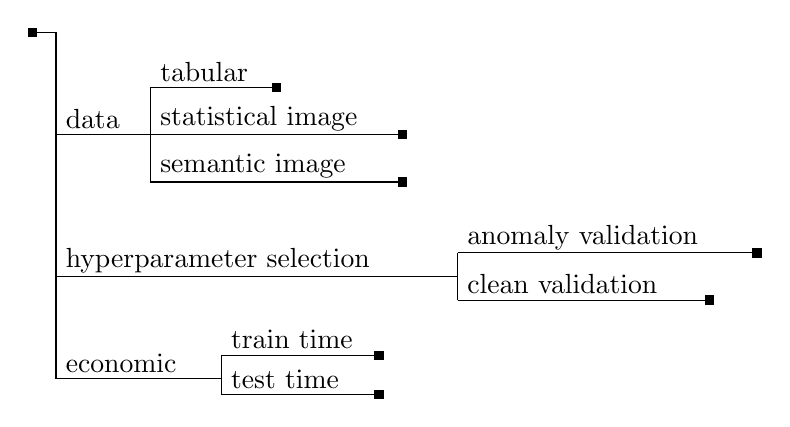
\begin{tikzpicture}
          \draw (-0.3,1.3) -- (0,1.3);
          \draw (0,1.3) -- (0,-3.1);
          
          \filldraw ([xshift=-1.5pt,yshift=-1.5pt]-0.3,1.3) rectangle ++(3pt,3pt);

          \draw (0,0) -- (1.2,0);
          \node[anchor=west] at (0,0.2) {data};
          \draw (1.2,-0.6) -- (1.2,0.6);
          \node[anchor=west] at (1.2,0.8) {tabular};
          \filldraw ([xshift=-1.5pt,yshift=-1.5pt]2.8,0.6) rectangle ++(3pt,3pt);
          \draw (1.2,0.6) -- (2.8,0.6);
          \node[anchor=west] at (1.2,0.2) {statistical image};
          \filldraw ([xshift=-1.5pt,yshift=-1.5pt]4.4,0) rectangle ++(3pt,3pt);
          \draw (1.2,0) -- (4.4,0);
          \node[anchor=west] at (1.2,-0.4) {semantic image};
          \filldraw ([xshift=-1.5pt,yshift=-1.5pt]4.4,-0.6) rectangle ++(3pt,3pt);
          \draw (1.2,-0.6) -- (4.4,-0.6);
          
          \draw (0,-1.8) -- (5.1,-1.8);
          \node[anchor=west] at (0,-1.6) {hyperparameter selection};
          \draw (5.1,-1.5) -- (5.1,-2.1);
          \filldraw ([xshift=-1.5pt,yshift=-1.5pt]8.9,-1.5) rectangle ++(3pt,3pt);
          \draw (5.1,-1.5) -- (8.9,-1.5);
          \node[anchor=west] at (5.1,-1.3) {anomaly validation};
          \filldraw ([xshift=-1.5pt,yshift=-1.5pt]8.3,-2.1) rectangle ++(3pt,3pt);
          \draw (5.1,-2.1) -- (8.3,-2.1);
          \node[anchor=west] at (5.1,-1.9) {clean validation};
          
          \draw (0,-3.1) -- (2.1,-3.1);
          \node[anchor=west] at (0,-2.9) {economic};
          \draw (2.1,-2.8) -- (2.1,-3.3);
          \filldraw ([xshift=-1.5pt,yshift=-1.5pt]4.1,-2.8) rectangle ++(3pt,3pt);
          \draw (2.1,-2.8) -- (4.1,-2.8);
          \node[anchor=west] at (2.1,-2.6) {train time};
          \filldraw ([xshift=-1.5pt,yshift=-1.5pt]4.1,-3.3) rectangle ++(3pt,3pt);
          \draw (2.1,-3.3) -- (4.1,-3.3);
          \node[anchor=west] at (2.1,-3.1) {test time};
          

    \end{tikzpicture}
    
    \caption{Various aspects of anomaly detection comparison forming the context of an experiment.}
    \label{fig:context}
\end{figure}

While many practitioners are eager to see which method is the best for their application, the specifics of the application may differ. In this chapter, a large number of experiments is conducted in order to identify the main sources of variability influencing the performance of anomaly detection methods. The number of combinations of these aspects is huge. Therefore, we have chosen the key axes of variability: datasets, hyperparameter selection strategy, and economic point of view. From these axes, we select a few discrete points, on which we will provide a comparison. The particular combination of the selected aspects will be called \textbf{context}, see Fig.~\ref{fig:context} for illustration. 

The first axis is the target data domain. Our experiments use two types of datasets: \textbf{tabular} and \textbf{image}. This is the most obvious split, and indeed most authors of prior art test their methods on either choice of data. Another possible way to look at data is whether they contain \textbf{statistical} or \textbf{semantic} anomalies, see Sec.~\ref{sec:ad_definition}. Statistical anomalies should be located in areas of a low likelihood of the normal class, while semantic~\cite{ahmed2020detecting} anomalies cannot be differentiated from normal data statistically. This is because they appear in datasets with multiple sources of variations, where only some of them are considered anomalous. Such types of anomalies are most common in image datasets. The suitability of the compared methods for the dataset context axis is studied in Sec.~\ref{sec:dataset_context}.

The second axis of variability is the hyperparameter selection strategy. It should be a gold standard that the experiments are repeated on different splits of data to training, validation, and testing subsets, especially if the datasets are small. However, in most of the reviewed recent papers~\cite{liu2019generative,wang2020advae,schlegl2017unsupervised, akcay2018ganomaly, perera2019ocgan}, this procedure was not mentioned with the exception of~\cite{ruff2018deep}. Therefore, our comparison fills this gap. Also, it is important to define the nature of information available for the selection of the hyperparameters: it is indeed a very different task if there is some (often small) number of known anomalies in the validation dataset that can be used to choose hyperparameters by cross-validation or if the validation dataset is clean (i.e. it contains no anomalies). In our experience, the former case is more common. Our observations are summarised in Sec.~\ref{sec:hyperparameter_context}.

The third axis is the economic aspect of a problem. There might be serious computational restrictions present in solving real-life problems. One might then not opt for a method that promises state-of-the-art performance, but for another that reaches slightly worse performance but can be trained economically, and its performance is robust with regards to hyperparameter optimization. More details on this can be found in Sec.~\ref{sec:economic_context}.

\section{Experimental setup}
\label{sec:experimentalsetup}

In order to achieve a fair and robust comparison, a strict procedure for testing each model was followed, which is shortly described in this section. For more details, see the original publication~\cite{vskvara2021comparison}.

\subsection{Data}

Two criteria guided the choice of datasets (mainly the tabular ones): first, they ought to be publicly available, and second, they should appear in surveys or articles presenting new methods.  In total, we have collected $40$ tabular datasets, the majority of which came from the UCI repository~\cite{Dua:2019}. The complete listing of number of samples and dimensions in each dataset is recorded in Appendix~\ref{sec:datasets} and Tab.~\ref{tab:tabular_datasets}. Except for the ANNThyroid, Arrhytmia, HAR, HTRU2, KDD Cup 99 (small), Spambase, Mammography, and Seismic, where the anomaly class has a clear meaning (security incident or disease), we have followed the technique of~\cite{emmott2013systematic} for creating artificial datasets for anomaly detection tasks from classification datasets. More precisely, we have used only "easy" and "medium" anomalies, as "hard" and "very hard" are not truly anomalous in the sense of being statistically distinct from the normal class.

The number of image datasets used for the evaluation of deep models is limited, as there are very few publicly available image datasets designed purely for anomaly detection - MNIST-C~\cite{muMNISTCRobustnessBenchmark2019} and MVTec-AD~\cite{bergmann2019mvtec}. Only three subsets \textit{wood, grid, transistor} of the MVTec-AD dataset were used due to our computational constraints. These were chosen since they represent problems of various degrees of difficulty. Furthermore, we have extended these with artificially created anomaly datasets based on common image datasets MNIST~\cite{lecun2010mnist}, FashionMNIST~\cite{xiao2017fashion}, CIFAR10~\cite{krizhevsky2009learning}, and SVHN2~\cite{netzer2011reading}. These are also used for anomaly detection tasks in the prior art~\cite{perera2019ocgan, pidhorskyi2018generative, ruff2018deep}. Again, basic statistics on image datasets are shown in the appendix Tab.~\ref{tab:image_datasets}. In the setting of this whole work, a single class (of digits/objects) is considered normal and the rest anomalous. Therefore, one classification image dataset is transformed into ten different anomaly detection subdatasets. Since the MNIST, FashionMNIST, MVTec-AD, and MNISTC datasets have a rich and consistent number of samples in the normal class and clear anomalies, we consider them to be statistical anomalies. On the other hand, images in the majority of classes in CIFAR10 and SVHN2 have a strong background and are thus considered to contain semantic anomalies. This prior division is also supported by a different behavior of different methods as reported in the following text.

The normal data samples in each dataset were randomly split in 60\%/20\%/20\% ratios to train/validation/test subsets, respectively. Anomalous data samples were split such that 50\% were in the validation part and 50\% in the testing part, which means the training subset has not contained anomalous samples. \footnote{A training set without any anomalies is in practice very optimistic, but this decision removes another degree of freedom from the evaluation for the sake of clarity of results.} The proportion of anomalies that were used in the validation phase varied from zero to the selected 50\%. This was done five times to produce different folds in all tabular and small (MvTec-AD and MNIST-C) image datasets, but only once for other image datasets, as the folds would be very homogenous, see the original paper.

\subsection{Models and their hyperparameters} \label{sec:hyperparameteroptimization}
\begin{table}
    \centering
    \tabcolsep=0.1cm
    
    \begin{tabular}{cll|cll}
    \toprule
    \textbf{class} & \textbf{model} & \textbf{acronym} & \textbf{class} & \textbf{model} & \textbf{acronym}  \\\midrule
    
    \parbox[t]{2mm}{\multirow{3}{*}{\rotatebox[origin=c]{90}{flows}}} & MAF & maf & \parbox[t]{2mm}{\multirow{5}{*}{\rotatebox[origin=c]{90}{two-stage}}} & DAGMM & dgmm \\
        & RealNVP & rnvp & & DeepSVDD & dsvd \\
        & SPTN & sptn & & REPEN & rpn  \\
        & & & & VAE-kNN & vaek \\

    \parbox[t]{2mm}{\multirow{5}{*}{\rotatebox[origin=c]{90}{autoencoders}}} 
        & AAE & aae & & VAE-OC-SVM & vaeo \\
        & adVAE & avae & & & \\

        & GANomaly & gano & \parbox[t]{2mm}{\multirow{8}{*}{\rotatebox[origin=c]{90}{shallow}}} & ABOD & abod \\

        & skipGANomaly & skip & & HBOS & hbos \\
        & VAE & vae & & IsolationForest & if \\
        & WAE & wae & & kNN & knn \\
        & & & & LODA & loda \\
    \parbox[t]{2mm}{\multirow{3}{*}{\rotatebox[origin=c]{90}{gans}}}
        & fAnoGAN & fano & & LOF & lof \\ 
        & fmGAN & fmgn & & OC-SVM & osvm \\
        & GAN & gan & & PidForest & pidf \\
        & MOGAAL & mgal & \\
    
    \bottomrule
    \end{tabular}

    \vspace*{0.15cm}
    \caption{Overview of the main classes of compared methods and the acronyms used in the text.}
    \label{tab:model_acronyms_2col}
\end{table}

Since the number of tested models is quite large, Tab.~\ref{tab:model_acronyms_2col} offers their overview together with acronyms used in graphs and tables and also an orientational division of the models into separate categories. Most of the deep models were coded from scratch, since the original implementations were either missing or non-functional. Properly exploring the space of hyperparameters of all models is paramount to achieving fair and comparable experimental comparison, yet this is often superficially treated. Researchers often use default or recommended values ignoring that they are sub-optimal on datasets they use in their comparison. The conflicting results of the MOGAAL method in the original publication~\cite{liu2019generative} and in~\cite{wang2020advae} demonstrate our argument. Another prototypical example is OC-SVM, which is typically used with Gaussian kernel and with $\nu$ set to some default value, e.g. 0.05~\cite{pevny2016loda}, but can achieve better results with different kernels. The choice of hyperparameters in anomaly detection is everything but easy. But this means that the experimental settings should be set up such that all methods have been optimized equally. We conjecture that recommended and default values of hyperparameters are strongly correlated with the choice of evaluation datasets in the publications that recommend them.

In order to explore the hyperparameter space of each method properly, we have employed a random search over a predefined grid for each method. This allows the construction of sections through the space for sensitivity studies. Moreover, it is frequently more efficient than grid search~\cite{bergstra2012random} and more flexible. For each model, dataset, and repetition, we have sampled 100 configurations from corresponding sets and trained the models with them. A fixed time budget was also given for training of each model, which automatically penalizes complicated models, which might theoretically achieve great performance, but are too computationally demanding.

A thorough exploration of the hyperparameter selection context also requires changing the criteria of model selection. When anomalies are available for validation, we select hyperparameters maximizing the AUC on the validation set. For experiments with no available anomalies, we have decided on the following hyperparameter selection mechanism. For shallow methods, we have used default hyperparameter values from literature - either authors of the method recommended them, they were used in a survey, or are default in a given implementation. Their overview is found in~\cite{vskvara2021comparison}. For deep methods, this is unfortunately impossible since their hyperparameter space is much larger, and the values are usually tuned to a specific dataset. Therefore, to have a universal solution, we have selected the already trained and evaluated models based on the lowest average anomaly score on the clean validation data, i.e. valdiation data without anomalies. This approach is theoretically justified for models with proper likelihood. 

\section{Experimental results}
\label{sec:results}
Unless specified otherwise, the performance results are estimates of the AUC on the testing set and averaged over all folds of the random cross-validation repetitions. When ranks are reported, they are calculated by ordering methods on each dataset and calculating the average across them (as recommended in~\cite{demvsar2006statistical}). Hyperparameters are selected using the best average performance over the folds of the validation dataset.

\subsection{Dataset context}
\label{sec:dataset_context}

\begin{figure*}[h]
    \begin{tabular}{c c}
    \resizebox{0.5\columnwidth}{!}{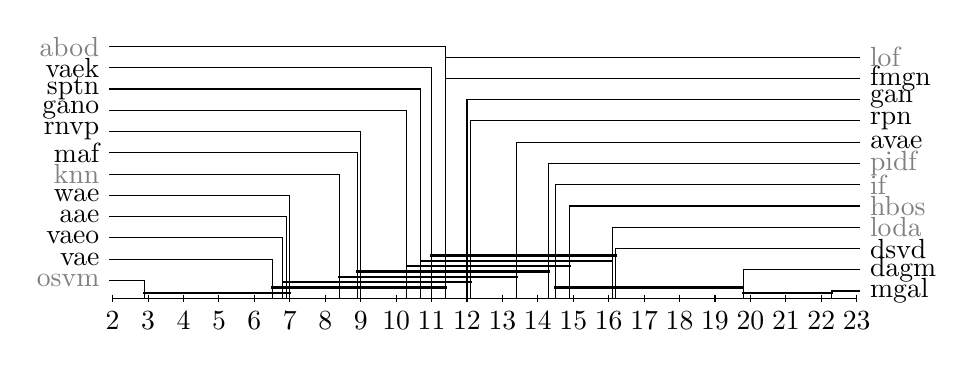
\begin{tikzpicture}[scale=0.45] 
  \draw (2.0,0) -- (23.0,0); 
  \foreach \x in {2,...,23} \draw (\x,0.10) -- (\x,-0.10) node[anchor=north]{$\x$}; 
  \draw (2.9,0) -- (2.9,0.5) -- (1.9, 0.5) node[anchor=east] {\textcolor{gray}{osvm}}; 
  \draw (6.5,0) -- (6.5,1.0999999999999999) -- (1.9, 1.0999999999999999) node[anchor=east] {vae}; 
  \draw (6.8,0) -- (6.8,1.6999999999999997) -- (1.9, 1.6999999999999997) node[anchor=east] {vaeo}; 
  \draw (6.9,0) -- (6.9,2.3) -- (1.9, 2.3) node[anchor=east] {aae}; 
  \draw (7.0,0) -- (7.0,2.9) -- (1.9, 2.9) node[anchor=east] {wae}; 
  \draw (8.4,0) -- (8.4,3.4999999999999996) -- (1.9, 3.4999999999999996) node[anchor=east] {\textcolor{gray}{knn}}; 
  \draw (8.9,0) -- (8.9,4.1000000000000005) -- (1.9, 4.1000000000000005) node[anchor=east] {maf}; 
  \draw (9.0,0) -- (9.0,4.7) -- (1.9, 4.7) node[anchor=east] {rnvp}; 
  \draw (10.3,0) -- (10.3,5.3) -- (1.9, 5.3) node[anchor=east] {gano}; 
  \draw (10.7,0) -- (10.7,5.9) -- (1.9, 5.9) node[anchor=east] {sptn}; 
  \draw (11.0,0) -- (11.0,6.5) -- (1.9, 6.5) node[anchor=east] {vaek}; 
  \draw (11.4,0) -- (11.4,7.1) -- (1.9, 7.1) node[anchor=east] {\textcolor{gray}{abod}}; 
  \draw (11.4,0) -- (11.4,6.8) -- (23.1, 6.8) node[anchor=west] {\textcolor{gray}{lof}}; 
  \draw (11.4,0) -- (11.4,6.2) -- (23.1, 6.2) node[anchor=west] {fmgn}; 
  \draw (12.0,0) -- (12.0,5.6) -- (23.1, 5.6) node[anchor=west] {gan}; 
  \draw (12.1,0) -- (12.1,5.0) -- (23.1, 5.0) node[anchor=west] {rpn}; 
  \draw (13.4,0) -- (13.4,4.4) -- (23.1, 4.4) node[anchor=west] {avae}; 
  \draw (14.3,0) -- (14.3,3.8) -- (23.1, 3.8) node[anchor=west] {\textcolor{gray}{pidf}}; 
  \draw (14.5,0) -- (14.5,3.2) -- (23.1, 3.2) node[anchor=west] {\textcolor{gray}{if}}; 
  \draw (14.9,0) -- (14.9,2.6) -- (23.1, 2.6) node[anchor=west] {\textcolor{gray}{hbos}}; 
  \draw (16.1,0) -- (16.1,1.9999999999999998) -- (23.1, 1.9999999999999998) node[anchor=west] {\textcolor{gray}{loda}}; 
  \draw (16.2,0) -- (16.2,1.4) -- (23.1, 1.4) node[anchor=west] {dsvd}; 
  \draw (19.8,0) -- (19.8,0.8) -- (23.1, 0.8) node[anchor=west] {dagm}; 
  \draw (22.3,0) -- (22.3,0.2) -- (23.1, 0.2) node[anchor=west] {mgal}; 
  \draw[line width=0.03cm,color=black,draw opacity=1.0] (2.87,0.15) -- (7.03,0.15); 
  \draw[line width=0.03cm,color=black,draw opacity=1.0] (6.47,0.3) -- (11.43,0.3); 
  \draw[line width=0.03cm,color=black,draw opacity=1.0] (6.77,0.44999999999999996) -- (12.129999999999999,0.44999999999999996); 
  \draw[line width=0.03cm,color=black,draw opacity=1.0] (8.370000000000001,0.6) -- (13.43,0.6); 
  \draw[line width=0.03cm,color=black,draw opacity=1.0] (8.870000000000001,0.75) -- (14.33,0.75); 
  \draw[line width=0.03cm,color=black,draw opacity=1.0] (10.270000000000001,0.9) -- (14.93,0.9); 
  \draw[line width=0.03cm,color=black,draw opacity=1.0] (10.67,1.05) -- (16.130000000000003,1.05); 
  \draw[line width=0.03cm,color=black,draw opacity=1.0] (10.97,1.2) -- (16.23,1.2); 
  \draw[line width=0.03cm,color=black,draw opacity=1.0] (14.47,0.3) -- (19.830000000000002,0.3); 
  \draw[line width=0.03cm,color=black,draw opacity=1.0] (19.77,0.15) -- (22.330000000000002,0.15); 
 \end{tikzpicture} 
} & \resizebox{0.5\columnwidth}{!}{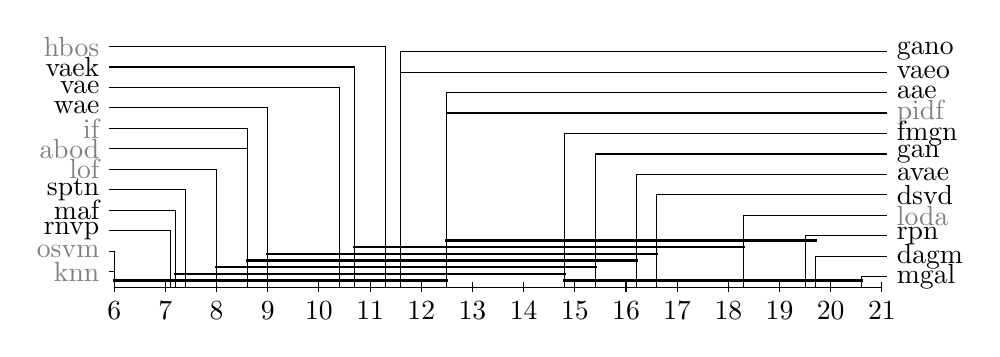
\begin{tikzpicture}[scale=0.65] 
  \draw (6.0,0) -- (21.0,0); 
  \foreach \x in {6,...,21} \draw (\x,0.10) -- (\x,-0.10) node[anchor=north]{$\x$}; 
  \draw (6.0,0) -- (6.0,0.30000000000000004) -- (5.9, 0.30000000000000004) node[anchor=east] {\textcolor{gray}{knn}}; 
  \draw (6.0,0) -- (6.0,0.7000000000000001) -- (5.9, 0.7000000000000001) node[anchor=east] {\textcolor{gray}{osvm}}; 
  \draw (7.1,0) -- (7.1,1.1) -- (5.9, 1.1) node[anchor=east] {rnvp}; 
  \draw (7.2,0) -- (7.2,1.5) -- (5.9, 1.5) node[anchor=east] {maf}; 
  \draw (7.4,0) -- (7.4,1.9) -- (5.9, 1.9) node[anchor=east] {sptn}; 
  \draw (8.0,0) -- (8.0,2.3000000000000003) -- (5.9, 2.3000000000000003) node[anchor=east] {\textcolor{gray}{lof}}; 
  \draw (8.6,0) -- (8.6,2.7) -- (5.9, 2.7) node[anchor=east] {\textcolor{gray}{abod}}; 
  \draw (8.6,0) -- (8.6,3.1) -- (5.9, 3.1) node[anchor=east] {\textcolor{gray}{if}}; 
  \draw (9.0,0) -- (9.0,3.5) -- (5.9, 3.5) node[anchor=east] {wae}; 
  \draw (10.4,0) -- (10.4,3.9) -- (5.9, 3.9) node[anchor=east] {vae}; 
  \draw (10.7,0) -- (10.7,4.300000000000001) -- (5.9, 4.300000000000001) node[anchor=east] {vaek}; 
  \draw (11.3,0) -- (11.3,4.700000000000001) -- (5.9, 4.700000000000001) node[anchor=east] {\textcolor{gray}{hbos}}; 
  \draw (11.6,0) -- (11.6,4.6000000000000005) -- (21.1, 4.6000000000000005) node[anchor=west] {gano}; 
  \draw (11.6,0) -- (11.6,4.2) -- (21.1, 4.2) node[anchor=west] {vaeo}; 
  \draw (12.5,0) -- (12.5,3.8000000000000003) -- (21.1, 3.8000000000000003) node[anchor=west] {aae}; 
  \draw (12.5,0) -- (12.5,3.4000000000000004) -- (21.1, 3.4000000000000004) node[anchor=west] {\textcolor{gray}{pidf}}; 
  \draw (14.8,0) -- (14.8,3.0000000000000004) -- (21.1, 3.0000000000000004) node[anchor=west] {fmgn}; 
  \draw (15.4,0) -- (15.4,2.6000000000000005) -- (21.1, 2.6000000000000005) node[anchor=west] {gan}; 
  \draw (16.2,0) -- (16.2,2.2) -- (21.1, 2.2) node[anchor=west] {avae}; 
  \draw (16.6,0) -- (16.6,1.8) -- (21.1, 1.8) node[anchor=west] {dsvd}; 
  \draw (18.3,0) -- (18.3,1.4000000000000001) -- (21.1, 1.4000000000000001) node[anchor=west] {\textcolor{gray}{loda}}; 
  \draw (19.5,0) -- (19.5,1.0) -- (21.1, 1.0) node[anchor=west] {rpn}; 
  \draw (19.7,0) -- (19.7,0.6000000000000001) -- (21.1, 0.6000000000000001) node[anchor=west] {dagm}; 
  \draw (20.6,0) -- (20.6,0.2) -- (21.1, 0.2) node[anchor=west] {mgal}; 
  \draw[line width=0.03cm,color=black,draw opacity=1.0] (5.97,0.13) -- (12.53,0.13); 
  \draw[line width=0.03cm,color=black,draw opacity=1.0] (7.17,0.26) -- (14.83,0.26); 
  \draw[line width=0.03cm,color=black,draw opacity=1.0] (7.97,0.39) -- (15.43,0.39); 
  \draw[line width=0.03cm,color=black,draw opacity=1.0] (8.57,0.52) -- (16.23,0.52); 
  \draw[line width=0.03cm,color=black,draw opacity=1.0] (8.97,0.65) -- (16.630000000000003,0.65); 
  \draw[line width=0.03cm,color=black,draw opacity=1.0] (10.67,0.78) -- (18.330000000000002,0.78); 
  \draw[line width=0.03cm,color=black,draw opacity=1.0] (12.47,0.91) -- (19.73,0.91); 
  \draw[line width=0.03cm,color=black,draw opacity=1.0] (14.770000000000001,0.13) -- (20.630000000000003,0.13); 
 \end{tikzpicture} 
} \\
    a) tabular, anomaly validation & b) tabular, clean validation \\  
    \resizebox{0.5\columnwidth}{!}{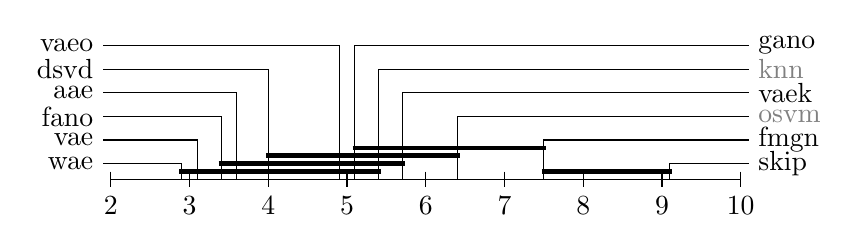
\begin{tikzpicture}[scale=1.0] 
  \draw (2.0,0) -- (10.0,0); 
  \foreach \x in {2,...,10} \draw (\x,0.10) -- (\x,-0.10) node[anchor=north]{$\x$}; 
  \draw (2.9,0) -- (2.9,0.19999999999999998) -- (1.9, 0.19999999999999998) node[anchor=east] {wae}; 
  \draw (3.1,0) -- (3.1,0.5) -- (1.9, 0.5) node[anchor=east] {vae}; 
  \draw (3.4,0) -- (3.4,0.7999999999999999) -- (1.9, 0.7999999999999999) node[anchor=east] {fano}; 
  \draw (3.6,0) -- (3.6,1.0999999999999999) -- (1.9, 1.0999999999999999) node[anchor=east] {aae}; 
  \draw (4.0,0) -- (4.0,1.4) -- (1.9, 1.4) node[anchor=east] {dsvd}; 
  \draw (4.9,0) -- (4.9,1.6999999999999997) -- (1.9, 1.6999999999999997) node[anchor=east] {vaeo}; 
  \draw (5.1,0) -- (5.1,1.7) -- (10.1, 1.7) node[anchor=west] {gano}; 
  \draw (5.4,0) -- (5.4,1.4) -- (10.1, 1.4) node[anchor=west] {\textcolor{gray}{knn}}; 
  \draw (5.7,0) -- (5.7,1.0999999999999999) -- (10.1, 1.0999999999999999) node[anchor=west] {vaek}; 
  \draw (6.4,0) -- (6.4,0.8) -- (10.1, 0.8) node[anchor=west] {\textcolor{gray}{osvm}}; 
  \draw (7.5,0) -- (7.5,0.5) -- (10.1, 0.5) node[anchor=west] {fmgn}; 
  \draw (9.1,0) -- (9.1,0.2) -- (10.1, 0.2) node[anchor=west] {skip}; 
  \draw[line width=0.06cm,color=black,draw opacity=1.0] (2.87,0.1) -- (5.430000000000001,0.1); 
  \draw[line width=0.06cm,color=black,draw opacity=1.0] (3.37,0.2) -- (5.73,0.2); 
  \draw[line width=0.06cm,color=black,draw opacity=1.0] (3.97,0.30000000000000004) -- (6.430000000000001,0.30000000000000004); 
  \draw[line width=0.06cm,color=black,draw opacity=1.0] (5.069999999999999,0.4) -- (7.53,0.4); 
  \draw[line width=0.06cm,color=black,draw opacity=1.0] (7.47,0.1) -- (9.129999999999999,0.1); 
 \end{tikzpicture} 
} & \resizebox{0.5\columnwidth}{!}{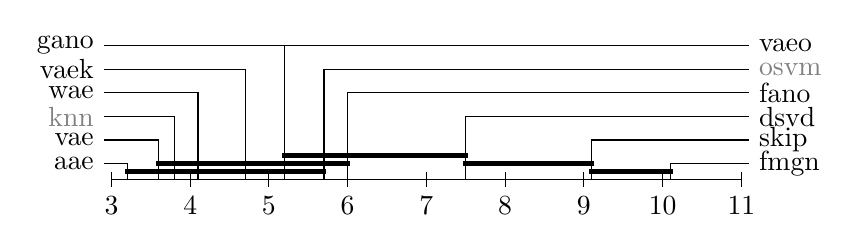
\begin{tikzpicture}[scale=1.0] 
  \draw (3.0,0) -- (11.0,0); 
  \foreach \x in {3,...,11} \draw (\x,0.10) -- (\x,-0.10) node[anchor=north]{$\x$}; 
  \draw (3.2,0) -- (3.2,0.19999999999999998) -- (2.9, 0.19999999999999998) node[anchor=east] {aae}; 
  \draw (3.6,0) -- (3.6,0.5) -- (2.9, 0.5) node[anchor=east] {vae}; 
  \draw (3.8,0) -- (3.8,0.7999999999999999) -- (2.9, 0.7999999999999999) node[anchor=east] {\textcolor{gray}{knn}}; 
  \draw (4.1,0) -- (4.1,1.0999999999999999) -- (2.9, 1.0999999999999999) node[anchor=east] {wae}; 
  \draw (4.7,0) -- (4.7,1.4) -- (2.9, 1.4) node[anchor=east] {vaek}; 
  \draw (5.2,0) -- (5.2,1.6999999999999997) -- (2.9, 1.6999999999999997) node[anchor=east] {gano}; 
  \draw (5.2,0) -- (5.2,1.7) -- (11.1, 1.7) node[anchor=west] {vaeo}; 
  \draw (5.7,0) -- (5.7,1.4) -- (11.1, 1.4) node[anchor=west] {\textcolor{gray}{osvm}}; 
  \draw (6.0,0) -- (6.0,1.0999999999999999) -- (11.1, 1.0999999999999999) node[anchor=west] {fano}; 
  \draw (7.5,0) -- (7.5,0.8) -- (11.1, 0.8) node[anchor=west] {dsvd}; 
  \draw (9.1,0) -- (9.1,0.5) -- (11.1, 0.5) node[anchor=west] {skip}; 
  \draw (10.1,0) -- (10.1,0.2) -- (11.1, 0.2) node[anchor=west] {fmgn}; 
  \draw[line width=0.06cm,color=black,draw opacity=1.0] (3.1700000000000004,0.1) -- (5.73,0.1); 
  \draw[line width=0.06cm,color=black,draw opacity=1.0] (3.5700000000000003,0.2) -- (6.03,0.2); 
  \draw[line width=0.06cm,color=black,draw opacity=1.0] (5.17,0.30000000000000004) -- (7.53,0.30000000000000004); 
  \draw[line width=0.06cm,color=black,draw opacity=1.0] (7.47,0.2) -- (9.129999999999999,0.2); 
  \draw[line width=0.06cm,color=black,draw opacity=1.0] (9.07,0.1) -- (10.129999999999999,0.1); 
 \end{tikzpicture} 
}\\
    c) statistical images, anomaly validation & d) statistical images, clean validation \\ 
     \resizebox{0.5\columnwidth}{!}{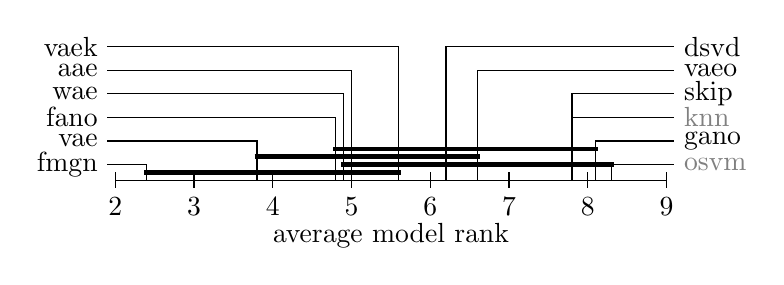
\begin{tikzpicture}[scale=1.0] 
  \draw (2.0,0) -- (9.0,0); 
  \foreach \x in {2,...,9} \draw (\x,0.10) -- (\x,-0.10) node[anchor=north]{$\x$}; 
  \draw (2.4,0) -- (2.4,0.19999999999999998) -- (1.9, 0.19999999999999998) node[anchor=east] {fmgn}; 
  \draw (3.8,0) -- (3.8,0.5) -- (1.9, 0.5) node[anchor=east] {vae}; 
  \draw (4.8,0) -- (4.8,0.7999999999999999) -- (1.9, 0.7999999999999999) node[anchor=east] {fano}; 
  \draw (4.9,0) -- (4.9,1.0999999999999999) -- (1.9, 1.0999999999999999) node[anchor=east] {wae}; 
  \draw (5.0,0) -- (5.0,1.4) -- (1.9, 1.4) node[anchor=east] {aae}; 
  \draw (5.6,0) -- (5.6,1.6999999999999997) -- (1.9, 1.6999999999999997) node[anchor=east] {vaek}; 
  \draw (6.2,0) -- (6.2,1.7) -- (9.1, 1.7) node[anchor=west] {dsvd}; 
  \draw (6.6,0) -- (6.6,1.4) -- (9.1, 1.4) node[anchor=west] {vaeo}; 
  \draw (7.8,0) -- (7.8,1.0999999999999999) -- (9.1, 1.0999999999999999) node[anchor=west] {skip}; 
  \draw (7.8,0) -- (7.8,0.8) -- (9.1, 0.8) node[anchor=west] {\textcolor{gray}{knn}}; 
  \draw (8.1,0) -- (8.1,0.5) -- (9.1, 0.5) node[anchor=west] {gano}; 
  \draw (8.3,0) -- (8.3,0.2) -- (9.1, 0.2) node[anchor=west] {\textcolor{gray}{osvm}}; 
  \draw[line width=0.06cm,color=black,draw opacity=1.0] (2.37,0.1) -- (5.63,0.1); 
  \draw[line width=0.06cm,color=black,draw opacity=1.0] (3.77,0.3) -- (6.63,0.3); 
  \draw[line width=0.06cm,color=black,draw opacity=1.0] (4.77,0.4) -- (8.129999999999999,0.4); 
  \draw[line width=0.06cm,color=black,draw opacity=1.0] (4.87,0.2) -- (8.33,0.2); 
  \node[anchor=center] at (5.5,-0.7) {average model rank};
 \end{tikzpicture} 
} & \resizebox{0.5\columnwidth}{!}{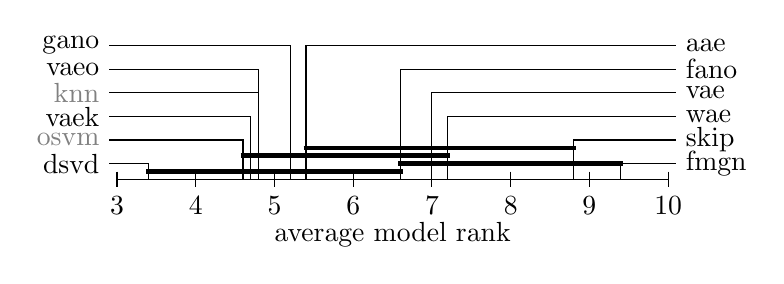
\begin{tikzpicture}[scale=1.0] 
  \draw (3.0,0) -- (10.0,0); 
  \foreach \x in {3,...,10} \draw (\x,0.10) -- (\x,-0.10) node[anchor=north]{$\x$}; 
  \draw (3.4,0) -- (3.4,0.19999999999999998) -- (2.9, 0.19999999999999998) node[anchor=east] {dsvd}; 
  \draw (4.6,0) -- (4.6,0.5) -- (2.9, 0.5) node[anchor=east] {\textcolor{gray}{osvm}}; 
  \draw (4.7,0) -- (4.7,0.7999999999999999) -- (2.9, 0.7999999999999999) node[anchor=east] {vaek}; 
  \draw (4.8,0) -- (4.8,1.0999999999999999) -- (2.9, 1.0999999999999999) node[anchor=east] {\textcolor{gray}{knn}}; 
  \draw (4.8,0) -- (4.8,1.4) -- (2.9, 1.4) node[anchor=east] {vaeo}; 
  \draw (5.2,0) -- (5.2,1.6999999999999997) -- (2.9, 1.6999999999999997) node[anchor=east] {gano}; 
  \draw (5.4,0) -- (5.4,1.7) -- (10.1, 1.7) node[anchor=west] {aae}; 
  \draw (6.6,0) -- (6.6,1.4) -- (10.1, 1.4) node[anchor=west] {fano}; 
  \draw (7.0,0) -- (7.0,1.0999999999999999) -- (10.1, 1.0999999999999999) node[anchor=west] {vae}; 
  \draw (7.2,0) -- (7.2,0.8) -- (10.1, 0.8) node[anchor=west] {wae}; 
  \draw (8.8,0) -- (8.8,0.5) -- (10.1, 0.5) node[anchor=west] {skip}; 
  \draw (9.4,0) -- (9.4,0.2) -- (10.1, 0.2) node[anchor=west] {fmgn}; 
  \draw[line width=0.06cm,color=black,draw opacity=1.0] (3.37,0.1) -- (6.63,0.1); 
  \draw[line width=0.06cm,color=black,draw opacity=1.0] (4.569999999999999,0.3) -- (7.23,0.3); 
  \draw[line width=0.06cm,color=black,draw opacity=1.0] (5.37,0.4) -- (8.83,0.4); 
  \draw[line width=0.06cm,color=black,draw opacity=1.0] (6.569999999999999,0.2) -- (9.43,0.2); 
  \node[anchor=center] at (6.5,-0.7) {average model rank};
 \end{tikzpicture} 
} \\
    e) semantic images, anomaly validation & f) semantic images, clean validation \\
    \end{tabular}
 \caption{Critical difference diagram of models ranked via the test AUC. Models whose performance is statistically indistinguishable have a difference of ranks under the critical value of the Nemenyi test $CD_{0.1}$ and are joined by a horizontal band. Results are presented for different types of datasets: tabular (Top row), image datasets with statistical anomalies (Middle row), and image datasets with semantic anomalies (Bottom row); and two different hyperparameter selection cases: using anomalies in validation (left) and using clean validation (right).
 }
 % $CD_{0.05}(24, 40) = 5.75$
 \label{fig:critical_diag}
\end{figure*}

The results of the experimental comparison on all dataset types are presented in the form of critical difference diagrams (CDD) as recommended by Dem\v{s}ar~\cite{demvsar2006statistical}, see Fig.~\ref{fig:critical_diag}. These diagrams show the average rank of detectors across the datasets together with a confidence band that indicates that a statistical test cannot reject the hypothesis that two detectors perform the same. What follows is a commentary on the influence of the datatype with respect to two types of hyperparameter selection strategies differing in the number of anomalies in the validation set as defined in Section~\ref{sec:contexts}: i) anomaly validation context, and ii) clean validation context.

\textbf{Tabular data:} OC-SVM performs the best and it is \emph{statistically better} than almost all detectors except autoencoder-based generative models and VAE combined with OC-SVM in the case of anomaly validation context. The first 11 places (roughly one half) belong to models that can be divided into three groups: (i) OC-SVM and its variants, which estimate a density level of a distribution; (ii) flow models and kNN, which estimate the pdf (un-normalized in case of kNN); (iii) and variants of autoencoders, where the reconstruction error is related to pdf as explained in Sec.~\ref{sec:vae_models}. The same types of methods occupy the top positions in the clean validation context, Fig.~\ref{fig:critical_diag}b), however in a different order. The best is the kNN (due to the simplicity of its hyperparameters), and all other pdf-modeling methods (flows) have improved relative to the anomaly validation context. The autoencoder-based methods moved beyond shallow methods (LOF, ABOD, IF). We believe that models in the lower half of the scale in both validation contexts are not suitable for detecting statistical anomalies. We cannot explain the poor performance of MOGAAL, DAGMM, and adVAE, and we attribute it to different experimental environment. DeepSVDD was primarily implemented for image problems, where it performs relatively well.

Moreover, differences in mean ranks of many models in Fig.~\ref{fig:critical_diag} are statistically insignificant at level $p=0.1$, which is disappointing. Assuming the ranks remain the same, another 51 datasets would be needed to make the difference between OC-SVM and VAE statistically significant on tabular data with 50\% anomalies. This indicates that the results are relatively noisy and can be easily changed for a different choice of datasets.

\textbf{Statistical image data:} WAE and VAE models have the best average rank when evaluated on statistical image data, although their lead is not statistically significant over most of the other models as is evident from Fig.~\ref{fig:critical_diag}c). The autoencoder-based methods (AAE,VAE,WAE) perform well also in the clean validation context, complemented by the kNN, Fig.~\ref{fig:critical_diag}d).

\textbf{Semantic image data:} A different story is told by Fig.~\ref{fig:critical_diag}e) where the ranking of methods on image datasets with semantic anomalies is dominated by fmGAN by a large margin in the anomaly validation context. However, it is also the worst method in the clean validation context. In an opposite manner, OC-SVM and kNN perform very poorly in the anomaly validation context, but they are among the best in the clean validation context.  The best performing method in the clean validation context is DeepSVDD~\cite{ruff2018deep}. We conjecture that the performance of the fmGAN is related to the variability of its training. With a sufficient number of anomalies in the validation set, it is possible to find one trained model that fits the problem.

\subsection{Hyperparameter selection context}
\label{sec:hyperparameter_context}
The influence of the hyperparameter selection procedure on the results in the previous section is now studied in detail for few selected methods. We choose only those that scored among the best in the previous section. First, we analyze the sensitivity of these methods to the number of anomalies in the validation set. Second, we study hyperparameter selection for two individual methods, variational autoencoder family and OC-SVM.

\subsubsection{Impact of the number of anomalies in the validation set}
\begin{figure*}[hbt!]
    \centering
    \resizebox {\linewidth}{!}{
    \begin{tikzpicture}[]
\begin{groupplot}[group style={vertical sep = 0.5cm, horizontal sep = 1.0cm, group size=3 by 1}]

\nextgroupplot [
  % legend style = {at={(0.3,1.30)}, anchor=west},
  ylabel = {avg. AUC},
  width=5cm, height=7cm, scale only axis=true, 
  xtick={1,2,3,4,5,6,7,8}, 
  xticklabels={clean,$PR@\%0.01$,$PR@\%0.1$,$PR@\%1$,$PR@\%5$,$PR@\%10$,$PR@\%20$,$AUC_{val}$},
  width=5cm, height=7cm, scale only axis=true,
  x tick label style={rotate=50,anchor=east},
  title = {(tabular)},
  % title style={at={(current bounding box.north)}, anchor=west},
]

\addplot+ coordinates {
  (1.0, 0.72375)
  (2.0, 0.762)
  (3.0, 0.754)
  (4.0, 0.8047500000000001)
  (5.0, 0.83925)
  (6.0, 0.844)
  (7.0, 0.8562500000000002)
  (8.0, 0.8845000000000001)
};

\addplot+ coordinates {
  (1.0, 0.607)
  (2.0, 0.52475)
  (3.0, 0.5587500000000001)
  (4.0, 0.5867500000000001)
  (5.0, 0.6585)
  (6.0, 0.71375)
  (7.0, 0.7232500000000001)
  (8.0, 0.7502500000000001)
};

\addplot+ coordinates {};

\addplot+ coordinates {
  (1.0, 0.6375)
  (2.0, 0.66375)
  (3.0, 0.6797500000000001)
  (4.0, 0.6940000000000001)
  (5.0, 0.75325)
  (6.0, 0.7837500000000001)
  (7.0, 0.8067500000000001)
  (8.0, 0.8380000000000001)
};

\addplot+ coordinates {
  (1.0, 0.8087500000000002)
  (2.0, 0.8290000000000001)
  (3.0, 0.8310000000000001)
  (4.0, 0.8329999999999999)
  (5.0, 0.8362499999999999)
  (6.0, 0.8357499999999998)
  (7.0, 0.8454999999999998)
  (8.0, 0.8517499999999998)
};

\addplot+ coordinates {
  (1.0, 0.8145)
  (2.0, 0.7222500000000001)
  (3.0, 0.7222500000000001)
  (4.0, 0.77225)
  (5.0, 0.8247500000000001)
  (6.0, 0.8727499999999999)
  (7.0, 0.8854999999999998)
  (8.0, 0.9112500000000001)
};

\addplot+ coordinates {
  (1.0, 0.7329999999999999)
  (2.0, 0.7945)
  (3.0, 0.7665)
  (4.0, 0.7812500000000001)
  (5.0, 0.8154999999999999)
  (6.0, 0.8247499999999999)
  (7.0, 0.8310000000000001)
  (8.0, 0.8714999999999999)
};

\addplot+ coordinates {
  (1.0, 0.7372500000000001)
  (2.0, 0.5530000000000002)
  (3.0, 0.5897500000000002)
  (4.0, 0.6622499999999999)
  (5.0, 0.7882499999999999)
  (6.0, 0.79475)
  (7.0, 0.84175)
  (8.0, 0.8825)
};

\addplot+ coordinates {
  (1.0, 0.7842499999999999)
  (2.0, 0.7955000000000002)
  (3.0, 0.7945)
  (4.0, 0.79525)
  (5.0, 0.826)
  (6.0, 0.836)
  (7.0, 0.853)
  (8.0, 0.8647499999999999)
};

\addplot+ coordinates {
  (1.0, 0.7967500000000001)
  (2.0, 0.7994999999999999)
  (3.0, 0.8039999999999999)
  (4.0, 0.7997500000000002)
  (5.0, 0.8217500000000001)
  (6.0, 0.82675)
  (7.0, 0.8344999999999999)
  (8.0, 0.8482500000000002)
};

% \legend{{}{aae}, {}{dsvd}, {}{fmgn}, {}{knn}, {}{osvm}, {}{vae}, {}{vaeo}, {}{wae}, {}{rnvp}}

\nextgroupplot [
  legend columns = -1,
  legend style = {at={(0.5,1.2)}, anchor=center},
  legend entries = {aae, dsvd, fano, fmgn, knn, osvm, vae, vaeo, wae, rnvp},
  width=5cm, height=7cm, scale only axis=true, 
  xtick={1,2,3,4,5,6,7,8}, 
  xticklabels={clean,$PR@\%0.01$,$PR@\%0.1$,$PR@\%1$,$PR@\%5$,$PR@\%10$,$PR@\%20$,$AUC_{val}$},
  width=5cm, height=7cm, scale only axis=true,
  x tick label style={rotate=50,anchor=east},
  title = {(statistical)},
  % title style={at={(current bounding box.north)}, anchor=west},
]

\addplot+ coordinates {
  (1.0, 0.8664864864864865)
  (2.0, 0.867837837837838)
  (3.0, 0.8791891891891892)
  (4.0, 0.8999999999999999)
  (5.0, 0.8981081081081083)
  (6.0, 0.8978378378378378)
  (7.0, 0.901891891891892)
  (8.0, 0.908918918918919)
};

\addplot+ coordinates {
  (1.0, 0.654054054054054)
  (2.0, 0.7918918918918918)
  (3.0, 0.8108108108108109)
  (4.0, 0.8327027027027026)
  (5.0, 0.841891891891892)
  (6.0, 0.8543243243243243)
  (7.0, 0.8597297297297297)
  (8.0, 0.8802702702702703)
};

\addplot+ coordinates {
  (1.0, 0.841891891891892)
  (2.0, 0.8527027027027027)
  (3.0, 0.8589189189189189)
  (4.0, 0.8727027027027027)
  (5.0, 0.8891891891891893)
  (6.0, 0.8959459459459459)
  (7.0, 0.9045945945945946)
  (8.0, 0.9275675675675675)
};

\addplot+ coordinates {
  (1.0, 0.5199999999999999)
  (2.0, 0.5445945945945946)
  (3.0, 0.5948648648648649)
  (4.0, 0.6775675675675675)
  (5.0, 0.73)
  (6.0, 0.7454054054054053)
  (7.0, 0.8075675675675675)
  (8.0, 0.8856756756756757)
};

\addplot+ coordinates {
  (1.0, 0.8262162162162162)
  (2.0, 0.8670270270270269)
  (3.0, 0.8708108108108108)
  (4.0, 0.8781081081081081)
  (5.0, 0.8781081081081081)
  (6.0, 0.8783783783783784)
  (7.0, 0.8799999999999999)
  (8.0, 0.8856756756756757)
};

\addplot+ coordinates {
  (1.0, 0.7997297297297298)
  (2.0, 0.7021621621621621)
  (3.0, 0.7032432432432432)
  (4.0, 0.7451351351351351)
  (5.0, 0.7983783783783783)
  (6.0, 0.8308108108108109)
  (7.0, 0.8394594594594594)
  (8.0, 0.8824324324324324)
};

\addplot+ coordinates {
  (1.0, 0.8856756756756757)
  (2.0, 0.7954054054054054)
  (3.0, 0.8127027027027027)
  (4.0, 0.828918918918919)
  (5.0, 0.8727027027027027)
  (6.0, 0.897027027027027)
  (7.0, 0.905945945945946)
  (8.0, 0.9205405405405408)
};

\addplot+ coordinates {
  (1.0, 0.8164864864864865)
  (2.0, 0.687027027027027)
  (3.0, 0.6967567567567567)
  (4.0, 0.7478378378378379)
  (5.0, 0.851081081081081)
  (6.0, 0.8794594594594595)
  (7.0, 0.9013513513513514)
  (8.0, 0.929189189189189)
};

\addplot+ coordinates {
  (1.0, 0.8916216216216215)
  (2.0, 0.8862162162162162)
  (3.0, 0.8986486486486487)
  (4.0, 0.8997297297297298)
  (5.0, 0.9183783783783783)
  (6.0, 0.9205405405405406)
  (7.0, 0.9224324324324323)
  (8.0, 0.9289189189189189)
};

% has to be set manually to match the marker style of the flow (9th in the entries bellow)
\addlegendimage{red,densely dashed,every mark/.append style={solid,fill=red!80!black},mark=diamond*} 
% \legend{{}{aae}, {}{dsvd}, {}{fano}, {}{fmgn}, {}{knn}, {}{osvm}, {}{vae}, {}{vaeo}, {}{wae}}

%%% the color 
% blue,every mark/.append style={fill=blue!80!black},mark=*\\
% red,every mark/.append style={fill=red!80!black},mark=square*\\
% brown!60!black,every mark/.append style={fill=brown!80!black},mark=otimes*\\
% black,mark=star\\
% blue,every mark/.append style={fill=blue!80!black},mark=diamond*\\
% red,densely dashed,every mark/.append style={solid,fill=red!80!black},mark=*\\
% brown!60!black,densely dashed,every mark/.append style={
% solid,fill=brown!80!black},mark=square*\\
% black,densely dashed,every mark/.append style={solid,fill=gray},mark=otimes*\\
% blue,densely dashed,mark=star,every mark/.append style=solid\\
% red,densely dashed,every mark/.append style={solid,fill=red!80!black},mark=diamond*\\

\nextgroupplot [
  % legend style = {at={(0.3,1.30)}, anchor=west},
  width=5cm, height=7cm, scale only axis=true, 
  xtick={1,2,3,4,5,6,7,8}, 
  xticklabels={clean,$PR@\%0.01$,$PR@\%0.1$,$PR@\%1$,$PR@\%5$,$PR@\%10$,$PR@\%20$,$AUC_{val}$},
  width=5cm, height=7cm, scale only axis=true,
  x tick label style={rotate=50,anchor=east},
  title = {(semantic)},
  % title style={at={(current bounding box.north)}, anchor=west},
]

\addplot+ coordinates {
  (1.0, 0.5649999999999998)
  (2.0, 0.584)
  (3.0, 0.5745000000000001)
  (4.0, 0.5934999999999999)
  (5.0, 0.6)
  (6.0, 0.6079999999999999)
  (7.0, 0.614)
  (8.0, 0.6224999999999999)
};

\addplot+ coordinates {
  (1.0, 0.5920000000000001)
  (2.0, 0.575)
  (3.0, 0.5685)
  (4.0, 0.5975000000000001)
  (5.0, 0.6250000000000001)
  (6.0, 0.6320000000000001)
  (7.0, 0.6325000000000001)
  (8.0, 0.638)
};

\addplot+ coordinates {
  (1.0, 0.5595000000000001)
  (2.0, 0.541)
  (3.0, 0.5544999999999999)
  (4.0, 0.5899999999999999)
  (5.0, 0.5955)
  (6.0, 0.61)
  (7.0, 0.633)
  (8.0, 0.6424999999999998)
};

\addplot+ coordinates {
  (1.0, 0.5)
  (2.0, 0.4885)
  (3.0, 0.49799999999999994)
  (4.0, 0.6194999999999999)
  (5.0, 0.6765)
  (6.0, 0.7)
  (7.0, 0.7249999999999999)
  (8.0, 0.729)
};

\addplot+ coordinates {
  (1.0, 0.5730000000000001)
  (2.0, 0.5834999999999999)
  (3.0, 0.5824999999999999)
  (4.0, 0.5890000000000001)
  (5.0, 0.5945)
  (6.0, 0.5985)
  (7.0, 0.599)
  (8.0, 0.6015)
};

\addplot+ coordinates {
  (1.0, 0.5760000000000001)
  (2.0, 0.5090000000000001)
  (3.0, 0.536)
  (4.0, 0.5625)
  (5.0, 0.5860000000000001)
  (6.0, 0.5925)
  (7.0, 0.5975000000000001)
  (8.0, 0.6045)
};

\addplot+ coordinates {
  (1.0, 0.552)
  (2.0, 0.5469999999999999)
  (3.0, 0.5625)
  (4.0, 0.5995000000000001)
  (5.0, 0.6210000000000002)
  (6.0, 0.6315000000000001)
  (7.0, 0.6315)
  (8.0, 0.6439999999999999)
};

\addplot+ coordinates {
  (1.0, 0.5735000000000001)
  (2.0, 0.558)
  (3.0, 0.5574999999999999)
  (4.0, 0.574)
  (5.0, 0.588)
  (6.0, 0.5994999999999999)
  (7.0, 0.6035000000000001)
  (8.0, 0.619)
};

\addplot+ coordinates {
  (1.0, 0.549)
  (2.0, 0.5820000000000002)
  (3.0, 0.5705)
  (4.0, 0.6065)
  (5.0, 0.614)
  (6.0, 0.615)
  (7.0, 0.625)
  (8.0, 0.6305)
};

\end{groupplot}

\end{tikzpicture}

    }
    \caption{Sensitivity of methods to the number of anomalies available in the validation set for hyperparameter selection visualized in terms of the achieved AUC aggregated over all datasets in each category (columns). The clean validation context is the left-most point on the x-axis, and the anomaly validation context (50\% of available anomalies) is the right-most point. The points in-between were obtained by selecting models with the highest precision on the reported portion (e.g. 5\%) of validation samples with the highest anomaly scores.} 
    \label{fig:combined_knowledge_rank_patn_auc_repre}
\end{figure*}

The process of hyperparameter selection described in Sec.~\ref{sec:hyperparameteroptimization} depends on the availability of examples of anomalies in the validation set (recall that it is assumed that the validation dataset does not contain unknown anomalous samples, i.e. is not contaminated). Fig.~\ref{fig:combined_knowledge_rank_patn_auc_repre} displays the influence of the number of anomalous samples in the validation set on a finer grid between the two contexts reported before.  Note that for the first point on the x-axis where the clean valdiation dataset was used, the mechanism of model selection was different from the rest of the graph. This is the reason for the significant difference between the clean context and the remaining points.

First, we observe that the quality of the models selected using anomalies improves with an increasing number of anomalous samples, which is expected. However, for a low number of anomalies, many methods perform significantly worse than in the case of the clean validation context. This behavior is notable across dataset types, especially for OC-SVM, and to some extent VAE. We conjecture that the hyperparameter selection procedure of those methods has a tendency to overfit, and its hyperparameters are not robust. In contrast to this, the performance of kNN, WAE, and RealNVP degrades slowly with the declining number of anomalies, which suggests that they are quite robust in difficult operating conditions. We attribute it to the fact that these methods are more exact in their estimation of data likelihood than the rest. 

Second, we notice that the experimental results on the semantic image datasets are generally poor, as the AUC of the best model (fmGAN) on CIFAR10 is 0.72 and similarly on SVHN2, where the best model achieved $0.74$. On the other hand, anomaly detection methods perform well on statistical image datasets. This indicates, contrary to popular belief that the models fail to learn or identify the important semantic information, or they consider different semantic information anomalous, and they should be told which semantic aspect of an image should be considered as an anomaly, as for example blurred images might be anomalous as well. Again, more detailed results, e.g. non-aggregated AUC values for individual datasets, or illustrative samples of detected anomalies can be found in the original publication~\cite{vskvara2021comparison}.

A practitioner might also desire a method robust with respect to a poor choice of hyperparameters.  In general, deep methods in our experiments have demonstrated higher variance, probably due to the large number of hyperparameters and stochasticity involved in their initialization and training via batched gradient optimization. In this respect, GAN-based models seem to be the least robust, which is in line with~\cite{deecke2018image} stating that GANs are not directly optimized for anomaly detection. This hints at the potential cost of hyperparameter optimization --- with higher performance variance, one is less likely to train a well-performing model in a given number of attempts. On the other hand, given enough labeled anomalies for hyperparameter selection, the fmGAN model gained a noticeable edge on semantic image anomalies. 

\subsubsection{Sensitivity Analysis of the VAE family}
\label{sec:vae_results}
The richness of the landscape of models that are based on the VAE is evident even from the relatively short overview in Sec.~\ref{sec:vae_models}. These methods form a whole family with multiple sources of variability: i) approximation of the likelihood in training (loss function), ii) the choice of latent prior, and iii) the anomaly score. We will analyze the sensitivity of the results to these choices on tabular data in the anomaly validation context. We focus on this family since most of the novel deep generative models for anomaly detection are based on the autoencoder architecture, as well as the novel model that is introduced in Chapter~\ref{sec:chapter_sgvaegan}. Additional degrees of freedom include the parametrization of variance of $p_{\vc{\theta}}(\vc{x}|\vc{z}),$ which was discussed already in Fig.~\ref{fig:betavae}. The variance can be either fixed (called VAE-constant), used in~\cite{yaoUnsupervisedAnomalyDetection2019, wang2020advae, ahnDeepGenerativeModelsBased2020}, a trainable scalar (called VAE-scalar), or a trainable full diagonal (called VAE-diagonal), used in~\cite{an2015variational,xu2018unsupervised, zenatiEfficientGANBasedAnomaly2018}. In the experiments, all three variations were tested on tabular data; however on image data, the full diagonal was skipped due to computational constraints (and in line with the prior art, where only scalar variance is used).

The overall comparison in Fig.~\ref{fig:critical_diag} revealed that WAE and vanilla VAE variants perform best. The other degrees of freedom, namely richness of prior, used anomaly score, and parametrization of the variance, were treated as hyperparameters. Fig.~\ref{fig:tabular_ae_only_box_auc_meanmax} extends the study by showing the distribution of ranks over tabular datasets for different variants of VAE, including GANomaly and adVAE. First, notice that the spread of the method's ranks over various datasets is significant, as even ranks of the best methods vary from 3 to 15. This means that the conclusions below need to be taken with a grain of salt, as the experimental results are extremely noisy.

The ELBO-based score~\eqref{eq:vae_loss},  -el, together with the orthogonal decomposition~\eqref{eq:jacodeco_basic} of the likelihood~\cite{pidhorskyi2018generative}, -jc, does not perform well. The sampled reconstruction error~\eqref{eq:score_sample}, \mbox{-rs}, almost always performs better than the usual reconstruction error, -rm, calculated according to~\eqref{eq:score_mean}. This demonstrates that the common approach of replacing the mean of the decoder with that of the encoder is inferior but computationally cheaper (see Tab.~\ref{tab:predict_times} with prediction times). The inclusion of the discriminator score in~\eqref{eq:aae_score}, -di, of AAE (an autoencoder combined with GAN) seems to be also on par with the MC estimate~\eqref{eq:score_sample}. 

From the same figure, we also conclude that the models modelling full diagonal in $p_{\vc{\theta}}(\vc{x}|\vc{z})$, -d-, seem to be better than the scalar, -s-, or constant, -c-, variants. This result is important, as many comparisons in the prior art use the VAE-constant, despite the version with full diagonal being discussed in the original publication~\cite{kingma2013auto}.

The rich prior distribution on the latent space proposed in \cite{tomczak2018vae}, VAMP, -v-, does not seem to give an advantage in the anomaly detection except in the AAE, although it performed quite well in the practical anomaly detection problem in Sec.~\ref{sec:alfven}. Similarly, recent variants adVAE and GANomaly do not seem to work well on the tabular data, but they were not evaluated on them in the original publications.

\begin{figure}
    \centering
    \small
    \begin{tikzpicture}
\begin{axis}[
	height=12cm,
	width=8cm,
	ymin=0, ymax=47,
	xmin=0, xmax=35,
	ytick={1,3,5,6,7,8,10,11,12,14,15,16,18,19,20,22,23,24,25,27,28,29,31,32,33,35,36,37,39,40,42,43,45,46},
	yticklabels={avae,gano,aae-s-di,aae-s-jc,aae-s-rm,aae-s-rs,aae-sv-di,aae-sv-rm,aae-sv-rs,aae-d-di,aae-d-rm,aae-d-rs,aae-dv-di,aae-dv-rm,aae-dv-rs,vae-s-el,vae-s-jc,vae-s-rm,vae-s-rs,vae-d-el,vae-d-rm,vae-d-rs,vae-c-el,vae-c-rm,vae-c-rs,wae-s-jc,wae-s-rm,wae-s-rs,wae-sv-rm,wae-sv-rs,wae-d-rm,wae-d-rs,wae-dv-rm,wae-dv-rs}
	]
\addplot [fill=lightgray, boxplot prepared={
draw position=1,
lower whisker=34, lower quartile=13.75,
median=21.5, upper quartile=28.25,
upper whisker=34},
] coordinates {};
\addplot [fill=lightgray, boxplot prepared={
draw position=3,
lower whisker=34, lower quartile=3.75,
median=15.0, upper quartile=23.5,
upper whisker=34},
] coordinates {};
\addplot [fill=lime, boxplot prepared={
draw position=5,
lower whisker=30, lower quartile=6.0,
median=12.0, upper quartile=21.25,
upper whisker=30},
] coordinates {};
\addplot [fill=orange, boxplot prepared={
draw position=6,
lower whisker=34, lower quartile=11.5,
median=21.5, upper quartile=26.75,
upper whisker=34},
] coordinates {};
\addplot [fill=cyan, boxplot prepared={
draw position=7,
lower whisker=33, lower quartile=9.0,
median=16.5, upper quartile=24.25,
upper whisker=33},
] coordinates {};
\addplot [fill=red, boxplot prepared={
draw position=8,
lower whisker=31, lower quartile=6.0,
median=16.0, upper quartile=22.25,
upper whisker=31},
] coordinates {};
\addplot [fill=lime, boxplot prepared={
draw position=10,
lower whisker=32, lower quartile=7.75,
median=12.5, upper quartile=22.25,
upper whisker=32},
] coordinates {};
\addplot [fill=cyan, boxplot prepared={
draw position=11,
lower whisker=34, lower quartile=8.75,
median=15.0, upper quartile=21.75,
upper whisker=34},
] coordinates {};
\addplot [fill=red, boxplot prepared={
draw position=12,
lower whisker=31, lower quartile=5.0,
median=12.0, upper quartile=21.25,
upper whisker=31},
] coordinates {};
\addplot [fill=lime, boxplot prepared={
draw position=14,
lower whisker=34, lower quartile=5.5,
median=23.0, upper quartile=32.0,
upper whisker=34},
] coordinates {};
\addplot [fill=cyan, boxplot prepared={
draw position=15,
lower whisker=31, lower quartile=12.75,
median=20.0, upper quartile=25.0,
upper whisker=31},
] coordinates {};
\addplot [fill=red, boxplot prepared={
draw position=16,
lower whisker=31, lower quartile=7.0,
median=14.5, upper quartile=21.25,
upper whisker=31},
] coordinates {};
\addplot [fill=lime, boxplot prepared={
draw position=18,
lower whisker=34, lower quartile=3.0,
median=26.0, upper quartile=33.25,
upper whisker=34},
] coordinates {};
\addplot [fill=cyan, boxplot prepared={
draw position=19,
lower whisker=33, lower quartile=10.75,
median=19.0, upper quartile=27.25,
upper whisker=33},
] coordinates {};
\addplot [fill=red, boxplot prepared={
draw position=20,
lower whisker=33, lower quartile=7.0,
median=15.0, upper quartile=25.25,
upper whisker=33},
] coordinates {};
\addplot [fill=magenta, boxplot prepared={
draw position=22,
lower whisker=32, lower quartile=5.0,
median=16.0, upper quartile=23.0,
upper whisker=32},
] coordinates {};
\addplot [fill=orange, boxplot prepared={
draw position=23,
lower whisker=33, lower quartile=11.5,
median=18.0, upper quartile=23.0,
upper whisker=33},
] coordinates {};
\addplot [fill=cyan, boxplot prepared={
draw position=24,
lower whisker=34, lower quartile=6.0,
median=12.5, upper quartile=23.0,
upper whisker=34},
] coordinates {};
\addplot [fill=red, boxplot prepared={
draw position=25,
lower whisker=31, lower quartile=3.0,
median=12.5, upper quartile=20.25,
upper whisker=31},
] coordinates {};
\addplot [fill=magenta, boxplot prepared={
draw position=27,
lower whisker=33, lower quartile=4.5,
median=9.0, upper quartile=22.0,
upper whisker=33},
] coordinates {};
\addplot [fill=cyan, boxplot prepared={
draw position=28,
lower whisker=33, lower quartile=2.0,
median=11.0, upper quartile=22.25,
upper whisker=33},
] coordinates {};
\addplot [fill=red, boxplot prepared={
draw position=29,
lower whisker=32, lower quartile=2.0,
median=5.5, upper quartile=20.0,
upper whisker=32},
] coordinates {};
\addplot [fill=magenta, boxplot prepared={
draw position=31,
lower whisker=34, lower quartile=10.5,
median=21.5, upper quartile=31.0,
upper whisker=34},
] coordinates {};
\addplot [fill=cyan, boxplot prepared={
draw position=32,
lower whisker=34, lower quartile=7.25,
median=9.0, upper quartile=18.25,
upper whisker=34},
] coordinates {};
\addplot [fill=red, boxplot prepared={
draw position=33,
lower whisker=33, lower quartile=7.75,
median=16.5, upper quartile=25.0,
upper whisker=33},
] coordinates {};
\addplot [fill=orange, boxplot prepared={
draw position=35,
lower whisker=34, lower quartile=11.25,
median=22.5, upper quartile=31.25,
upper whisker=34},
] coordinates {};
\addplot [fill=cyan, boxplot prepared={
draw position=36,
lower whisker=30, lower quartile=5.0,
median=11.5, upper quartile=18.25,
upper whisker=30},
] coordinates {};
\addplot [fill=red, boxplot prepared={
draw position=37,
lower whisker=33, lower quartile=3.0,
median=7.0, upper quartile=17.25,
upper whisker=33},
] coordinates {};
\addplot [fill=cyan, boxplot prepared={
draw position=39,
lower whisker=32, lower quartile=5.0,
median=10.0, upper quartile=20.25,
upper whisker=32},
] coordinates {};
\addplot [fill=red, boxplot prepared={
draw position=40,
lower whisker=31, lower quartile=3.0,
median=7.0, upper quartile=15.25,
upper whisker=31},
] coordinates {};
\addplot [fill=cyan, boxplot prepared={
draw position=42,
lower whisker=31, lower quartile=2.0,
median=7.5, upper quartile=18.0,
upper whisker=31},
] coordinates {};
\addplot [fill=red, boxplot prepared={
draw position=43,
lower whisker=31, lower quartile=2.0,
median=6.0, upper quartile=15.75,
upper whisker=31},
] coordinates {};
\addplot [fill=cyan, boxplot prepared={
draw position=45,
lower whisker=33, lower quartile=6.0,
median=10.5, upper quartile=17.25,
upper whisker=33},
] coordinates {};
\addplot [fill=red, boxplot prepared={
draw position=46,
lower whisker=33, lower quartile=3.0,
median=7.0, upper quartile=13.0,
upper whisker=33},
] coordinates {};
\end{axis}
\end{tikzpicture}

    \caption{Sensitivity study of various variants of  autoencoder-based methods displayed in the form of boxplots of their ranks in the AUC metric achieved on the tabular datasets. The first three letters of the method's name denote the training loss. Models with the -d- middle part estimate full diagonal of the decoder variance, -s- estimate only a scalar, and -c-  use a fixed scalar variance as a hyperparameter. All variants are using the standard Gaussian latent model. Models using the VampPrior are denoted by extending the decoder variance symbol by the letter v-, i.e. -dv-, -sv-, -cv-. The last part of the name denotes score, -rs stands for the sampled rec. probability~\eqref{eq:score_sample} with $L=100$, -rm for~\eqref{eq:score_mean}, -el for the ELBO~\eqref{eq:vae_loss} composed of -rs and KLD, -jc for~\eqref{eq:jacodeco_basic}, -di for~\eqref{eq:aae_score}.}
    \label{fig:tabular_ae_only_box_auc_meanmax}
\end{figure}


\begin{table}
    \footnotesize
    \centering
    \tabcolsep=0.05cm
    \begin{tabular}{c|c c c c c}
         & vae-s-rs & vae-d-rs & vae-s-rm & vae-d-rm & vae-d-jc \\
         \midrule
        $\bar{t}_{pred}$ [s] & 12.10 & 18.51 & 0.11 & 0.15 & 57.31
    \end{tabular}
    \vspace*{0.15cm}
    \caption{Average prediction times on the  tabular datasets for different combinations of VAE scores and decoder variance estimations. The -d- part stands for model with an estimate of the full diagonal of the decoder variance, -s- is a scalar estimate. Sampled reconstruction error~\eqref{eq:score_sample} is denoted as -rs, -rm is the anomaly score~\eqref{eq:score_mean} and -jc is~\eqref{eq:jacodeco_basic}.}
    \label{tab:predict_times}
\end{table}


\subsubsection{Sensitivity study of OC-SVM}
\label{sub:OC-SVM}
This result on the optimization of OC-SVM, taken from~\cite{vskvara2021comparison}, is not directly related to the main result presented in Chapter~\ref{sec:chapter_sgvaegan}, but we found it interesting enough to include it in this compilation. The domination of OC-SVM on tabular data in anomaly validation context contrasts to many prior experimental comparisons~\cite{goldstein2016comparative, chalapathyGroupAnomalyDetection2018, deecke2018image, gopalanPIDForestAnomalyDetection2019, iwataSupervisedAnomalyDetection2019, wang2020advae}. The search for the culprit found it to be the hyperparameter selection. This study has varied the $\nu$ parameter, kernels, and their parameters, which is much more than the most prior art does, which is fixing the kernel to RBF and testing few values of its width $\gamma$ and $\nu.$ Inclusion of other kernels into the search for hyperparameters seems to be the major source of improvement in this case. Replacing the OC-SVM with one restricted to use only the RBF kernel and $\nu=0.5$ yields an increase in average rank from $2.9$ to $8.1$ with an average decrease in performance by $0.06$, measured in AUC in the anomaly validation context. This version of OC-SVM is then easily surpassed by variational autoencoders and kNN, as demonstrated in~\cite{vskvara2021comparison}.  The importance of the choice of the kernel is furthermore illustrated by the fact that the sigmoid kernel was the optimal choice for 23 datasets, while the RBF kernel was optimal only for 13. Ref.~\cite{goldstein2016comparative} mentions that setting $\nu=0.5$ provides universally good results, which may be the reason why many authors do not tune it. In theory, it should be set to much lower values ($\nu = 0.05$) corresponding to the presumed low ratio of anomalies in data, but with Bayesian optimization, we found that the best estimate of $\nu$ was in some cases even higher, such as $\sim0.75$ on the statlog-vehicle dataset.

\subsection{Economic context}
\label{sec:economic_context}
\begin{figure*}
    \centering
    \begin{subfigure}{\columnwidth}
        \centering
        \small
        \resizebox {0.66\linewidth}{!}{
            \begin{tikzpicture}[]
\begin{groupplot}[group style={vertical sep = 0.0cm, horizontal sep = 0.2cm, group size=2 by 1}]

\nextgroupplot [
  xlabel = {avg. rank},
  ylabel = {avg. training time rank},
  ylabel near ticks, yticklabel pos=left,
  ymin = 0.5, ymax=25,
  width=4cm, height=6cm, scale only axis=true,
  grid=major,
  % title = {(fit time)}
]

\addplot+[
  draw = none
] coordinates {
  (6.9, 11.3)
  (11.4, 8.8)
  (13.4, 12.7)
  (19.8, 16.2)
  (16.2, 10.9)
  (11.4, 18.8)
  (12.0, 16.2)
  (10.3, 9.7)
  (14.9, 4.4)
  (14.5, 5.0)
  (8.4, 2.4)
  (16.1, 3.4)
  (11.4, 2.6)
  (8.9, 21.8)
  % (22.3, 19.4)
  (2.9, 3.4)
  (14.3, 15.1)
  (9.0, 23.3)
  (12.1, 7.6)
  (10.7, 23.0)
  (6.5, 12.1)
  (11.0, 16.3)
  (6.8, 14.9)
  (7.0, 20.1)
};

\node at (axis cs:8.2, 12.0) {aae};

\node at (axis cs:13.1, 9.7) {abod};

\node at (axis cs:13.9, 13.3) {avae};

\node at (axis cs:18.9, 16.9) {dagm};

\node at (axis cs:16.7, 11.8) {dsvd};

\node at (axis cs:11.9, 19.5) {fmgn};

\node at (axis cs:13.0, 17.0) {gan};

\node at (axis cs:10.8, 10.3) {gano};

\node at (axis cs:16.8, 5.1) {hbos};

\node at (axis cs:14.1, 5.8) {if};

\node at (axis cs:8.8, 3.2) {knn};

\node at (axis cs:17.8, 2.9) {loda};

\node at (axis cs:11.6, 3.4) {lof};

\node at (axis cs:11.0, 21.8) {maf};

% \node at (axis cs:22.8, 20.0) {mgal};

\node at (axis cs:3.4, 4.1) {osvm};

\node at (axis cs:14.8, 15.7) {pidf};

\node at (axis cs:9.1, 24.0) {rnvp};

\node at (axis cs:13.6, 8.0) {rpn};

\node at (axis cs:12.8, 23.7) {sptn};

\node at (axis cs:7.0, 12.7) {vae};

\node at (axis cs:9.3, 17.0) {vaek};

\node at (axis cs:7.3, 15.6) {vaeo};

\node at (axis cs:7.5, 20.8) {wae};

\nextgroupplot [
  xlabel = {avg. rank},
  ylabel = {avg. prediction time rank},
  ylabel near ticks, yticklabel pos=right,
  ymin = 0.5, ymax=25,
  width=4cm, height=6cm, scale only axis=true,
  % title = {(evaluation time)},
  grid=major,
  % yticklabels={}
]

\addplot+[
  draw = none
] coordinates {
  (6.9, 13.3)    
  (11.4, 23.8)    
  (13.4, 21.8)
  (19.8, 1.3)
  (16.2, 7.0)
  (11.4, 2.3)
  (12.0, 2.2)
  (10.3, 5.6)
  (14.9, 4.4)
  (14.5, 16.0)
  (8.4, 15.1)
  (16.1, 10.4)
  (11.4, 11.5)
  (8.9, 12.2)
  % (22.3, 10.0)
  (2.9, 10.1)
  (14.3, 22.6)
  (9.0, 8.7)
  (12.1, 10.5)
  (10.7, 17.0)
  (6.5, 18.4)
  (11.0, 18.0)
  (6.8, 14.5)
  (7.0, 19.1)
};

\node at (axis cs:5.5, 13.8) {aae};

\node at (axis cs:11.9, 24.5) {abod};

\node at (axis cs:11.9, 22.4) {avae};

\node at (axis cs:18.3, 2.0) {dagm};

\node at (axis cs:16.7, 7.8) {dsvd};

\node at (axis cs:10.0, 3.0) {fmgn};

\node at (axis cs:13.5, 2.9) {gan};

\node at (axis cs:10.8, 6.3) {gano};

\node at (axis cs:15.4, 5.2) {hbos};

\node at (axis cs:15.1, 16.8) {if};

\node at (axis cs:8.9, 16.0) {knn};

\node at (axis cs:16.6, 11.2) {loda};

\node at (axis cs:12.3, 12.3) {lof};

\node at (axis cs:9.4, 12.8) {maf};

% \node at (axis cs:22.8, 10.7) {mgal};

\node at (axis cs:3.4, 10.7) {osvm};

\node at (axis cs:14.8, 23.3) {pidf};

\node at (axis cs:9.5, 9.3) {rnvp};

\node at (axis cs:13.7, 9.8) {rpn};

\node at (axis cs:8.9, 17.5) {sptn};

\node at (axis cs:5.0, 19.0) {vae};

\node at (axis cs:11.5, 18.9) {vaek};

\node at (axis cs:6.0, 15.2) {vaeo};

\node at (axis cs:5.5, 19.8) {wae};

\end{groupplot}
\end{tikzpicture}


        }
        \caption{tabular datasets}
        \label{fig:tabular_total_eval_t_fit_t_combined}
    \end{subfigure}
    \begin{subfigure}{\columnwidth}
        \centering
        \small
        \resizebox {0.66\linewidth}{!}{
            \begin{tikzpicture}[]
\begin{groupplot}[group style={vertical sep = 0.0cm, horizontal sep = 0.2cm, group size=2 by 1}]

\nextgroupplot [
  xlabel = {avg. rank},
  ylabel = {avg. training time rank},
  ylabel near ticks, yticklabel pos=left,
  ymin = 0.5, ymax=13,
  width=4cm, height=6cm, scale only axis=true,
  grid=major,
  % title = {(fit time)}
]

\addplot+[
  draw = none
] coordinates {
  (4.1, 5.0)
  (4.8, 6.5)
  (3.8, 11.8)
  (5.7, 11.2)
  (6.2, 6.8)
  (6.2, 1.6)
  (7.1, 1.8)
  (8.6, 5.2)
  (3.4, 7.3)
  (5.7, 5.4)
  (5.5, 5.6)
  (3.6, 9.9)
};

\node at (axis cs:4.4, 5.5) {aae};

\node at (axis cs:5.0, 7.0) {dsvd};

\node at (axis cs:4.3, 12.3) {fano};

\node at (axis cs:6.2, 11.7) {fmgn};

\node at (axis cs:6.6, 7.3) {gano};

\node at (axis cs:6.0, 2.2) {knn};

\node at (axis cs:7.6, 2.2) {osvm};

\node at (axis cs:8.2, 5.8) {skip};

\node at (axis cs:3.7, 7.8) {vae};

\node at (axis cs:6.5, 5.5) {vaek};

\node at (axis cs:6.1, 5.8) {vaeo};

\node at (axis cs:3.9, 10.4) {wae};

\nextgroupplot [
  xlabel = {avg. rank},
  ylabel = {avg. prediction time rank},
  ylabel near ticks, yticklabel pos=right,
  ymin = 0.5, ymax=13,
  width=4cm, height=6cm, scale only axis=true,
  % title = {(evaluation time)},
  grid=major,
  % yticklabels={}
]

\addplot+[
  draw = none
] coordinates {
  (4.1, 7.6)
  (4.8, 2.4)
  (3.8, 8.8)
  (5.7, 1.0)
  (6.2, 4.8)
  (6.2, 11.1)
  (7.1, 11.3)
  (8.6, 3.8)
  (3.4, 4.6)
  (5.7, 7.7)
  (5.5, 9.6)
  (3.6, 5.5)
};

\node at (axis cs:4.4, 8.1) {aae};

\node at (axis cs:5.3, 3.1) {dsvd};

\node at (axis cs:4.3, 9.5) {fano};

\node at (axis cs:6.2, 1.7) {fmgn};

\node at (axis cs:6.7, 5.3) {gano};

\node at (axis cs:6.0, 11.6) {knn};

\node at (axis cs:7.4, 11.8) {osvm};

\node at (axis cs:8.5, 4.5) {skip};

\node at (axis cs:3.9, 5.0) {vae};

\node at (axis cs:6.2, 8.4) {vaek};

\node at (axis cs:6.0, 10.0) {vaeo};

\node at (axis cs:4.1, 6.0) {wae};

\end{groupplot}
\end{tikzpicture}


        }
        \caption{image datasets}
        \label{fig:images_total_eval_t_fit_t_combined}
    \end{subfigure}
    \caption{Scatter-plots of the average rank in the AUC metric on the tabular  (a) and image (b) data versus average rank of the computational complexity of the displayed methods measured via training time (left) and prediction time (right). MO-GAAL has been omitted from the tabular figures, as its performance positioned it too far to the right with the training time rank of $19.4$ and the prediction time rank of $10.0$.}
    \label{fig:images_total_eval_t_fit_t_combined_joined}
\end{figure*}

Practitioners ask for fast and accurate algorithms, but these two features rarely go hand in hand, and a decision on a trade-off has to be made. When one plots model performance against computational intensity, the interesting methods lie on the Pareto frontier~\cite{ishizaka2013multi}, as in the absence of an external factor, rationally behaving practitioner does not have a motivation to choose a different model.

Fig.~\ref{fig:tabular_total_eval_t_fit_t_combined}-left shows the trade-off between accuracy and training time for tabular data, where the absolute numbers were replaced by average ranks for robustness. The Pareto frontier contains two methods, which are OC-SVM and kNN. The position of OC-SVM is rather surprising, as its training time is known to scale poorly (quadratically) with respect to the number of samples, but it is caused by most of the tabular datasets being small. Different results may arise for a dataset with many data records. Fig.~\ref{fig:tabular_total_eval_t_fit_t_combined}-right shows a similar trade-off between accuracy and testing (inference) time. OC-SVM is still on the Pareto frontier, but it is expensive, as the complexity grows linearly in the number of samples. fmGAN, GAN and DAGMM methods are there as well -- these methods have fast inference but lower accuracy.

We provide results averaged over the studied contexts on image data. Due to the variability of the results in each context, the x-axis will vary. In the averaged ranks, VAE is on the Pareto front in both fit and prediction times, see Fig.~\ref{fig:images_total_eval_t_fit_t_combined}. Its prediction complexity is given mainly by choice of the number of samples taken in the computation of the sampled reconstruction score~\eqref{eq:score_sample}. The kNN detector has negligible training time, given only by the construction of the tree structure representing data, but seems to be mostly unusable on image data due to slow prediction times on datasets that are large in dimension and number of samples. The fmGAN finds itself in a completely reversed scenario.

\section{Conclusion}
The presented extensive comparison of anomaly detection methods based on deep generative methods, namely variants of flows, variational autoencoders, and generative adversarial networks with shallow methods based on alternative paradigms revealed that the performance of anomaly detection methods strongly depends on experimental conditions. We have identified the most important contexts (sources of variation) to be the type of data, availability of labeled anomalies for hyperparameter tuning and of course the available computational power. There are also factors of variance that have a smaller relevance in the conducted experiments in~\cite{vskvara2021comparison}, such as the use of ensembles, alternative performance metrics and Bayesian optimization of model hyperparameters, which did not have an effect on the relative performance of different models.

This is the list of some of the most important practical observations and recommendations, some of which will be relevant in Chapter~\ref{chapter:sgvaegan}.
\begin{itemize}
    \item Methods with more exact likelihood modeling, such as kNN, flows, and autoencoder-based models, perform better in scenarios with a limited number of anomalies available for hyperparameter tuning.
    \item Majority of the methods fail to detect semantic anomalies. The exception is the fmGAN, which uses a generator-discriminator pair, but only if given enough computational resources and many anomalous samples for cross-validation. 
    \item OC-SVM, when properly tuned, can defeat most of the state-of-the-art on tabular data, although it suffers from overfitting when hyperparameters are selected using too few anomalies in the validation set.
    \item The method of the first choice appears to be the VAE/WAE due to its relatively cheap, precise, and consistent performance in most of the experiments. However, it possesses so many degrees of freedom that it forms a full family of methods. It was found that the best performance is obtained when estimating the full variance of samples on the output of the decoder and evaluating anomalies using sampled reconstruction score. 
\end{itemize}

Many aspects have not been covered and remain a topic of future work, such as the identification of the relevant kind of anomalies in the semantic datasets or the design of ensembles of methods of various types. Although we have shown that the number of anomalies available for validation is an important context, there was no further budget for a comparison of anomaly detection methods with active learning.  We have also completely left out the comparison of models on temporal data, such as time series or video, which is a very challenging task. Finally, an interesting area to study further is the influence of the presence of unlabeled anomalies in the training data.
